\section{Introduction}

This paper is a review of the systematic mapping study
``A Systematic Mapping Study on Microservices Architecture in DevOps'' \cite{waseem:SMSMSADevOps}.
The goal is to introduce the reader to the topic, explain the used
methods in empirical software engineering, and give a critical review
of the conducted study and the results.

The study used a broad search over several well-known publication-databases
and searched for research material on the topic of microservice architectures
in the DevOps context. After the first search, additional material
was searched for with a technique called ``snowballing''. All this material
was then screened and analyzed and after an initial selection was made,
the studies were fully read and information extracted. The results
are then mapped and categorized according to guidelines.

The study shows various problems and their corresponding solutions
along with some challenges (problems without any purposed solution).
Some of the problems do not have a solution because gray literature is
not allowed in the search.

The remainder of the paper will introduce terms and principles that are used
in the reviewed study, as well as topics that are needed for the understanding
of the study and this review. Furthermore, a neutral summary of the reviewed study
\cite{waseem:SMSMSADevOps} is provided. After the summary a critical review
is conducted and then a conclusion is derived from the previous sections.


\subsection{Design Science}

Design Science has the main purpose of achieving knowledge and a general understanding
about a domain \cite{hevner:DesignScience}. Design Science contains several guidelines
according to Alan R. Hevner (among other authors). Those guidelines are \cite{hevner:DesignScience}:

\begin{itemize}
    \item \textit{Design as an artefact}: Design Science must produce an artifact
    \item \textit{Problem relevance}: The objective is to develop solutions to relevant business problems
    \item \textit{Design evaluation}: The utility of an artifact must be demonstrated with evaluation methods
    \item \textit{Research contributions}: It must provide clear and verifiable contributions to the topic
    \item \textit{Research rigor}: The research relies on rigorous methods in construction and evaluation of the model
    \item \textit{Design as a search process}: The search for artifacts requires satisfying laws to be in place
    \item \textit{Communication of research}: The targeted audience should be technology-based as well as management based
\end{itemize}


\subsection{Empirical Software Engineering}

Empirical Software Engineering (ESE) provides a solid base for discussion and methods for empirical
research regarding software engineering topics. It has a strong emphasis on \textit{empirical}.

\subsubsection{Systematic Mapping Study (SMS)}

A SMS is a defined method to gather, analyze, classify, and structure a field of interest.
The result of an SMS allows readers and researchers to determine the coverage of the given
field of interest \cite{petersen:SMS}. The analysis focuses on frequency and topics for a
field. It is a defined process in which the following steps take place \cite{petersen:SMS}:

\begin{enumerate}
    \item Define research questions (RQs) and topic
    \item Define search query and parameter
    \item Search for articles and publications in given databases
    \item Analyze and screen the results (i.e., quality assessment and data analysing)
    \item Classify and map the given articles
\end{enumerate}

\subsubsection{Systematic Literature Review (SLR)}

A SLR is a method of ESE to systematically analyze and review a given topic. It uses
methods to collect secondary data and critically reviews the given research study.
The search for additional data can involve published as well as unpublished work
on the subject \cite{siddaway:SLR}.

\subsubsection{Systematic Gray Literature Review (SGLR)}

A SGLR is essentially the same as an SLR with a very important difference:
It does not only consider published and unpublished \textit{peer reviewed} work,
but also ``Gray Literature''. Gray literature is evidence and material that
is not published in commercial and peer reviewed publications \cite{paez:GrayLiterature}.
In the context of computer science, gray literature can provide important statements
and evidence towards topics that are more driven by businesses than by the academia.


\subsection{Microservices and DevOps}

Since the topic of the reviewed paper does conduct an SMS over ``Microservices in DevOps'',
it is utterly important to define those terms so that any reader of this paper
understands the base of the terms on which the conclusions are built upon.

\subsubsection{Microservices}

Microservices (sometimes referred to as ``Microservice Architecture'') is an application
structural style. The style focuses on building several small services that cooperate
together to create an application \cite{richardson:whatIsMSA}. Those services are often deployed on distributed
systems. Most microservices adhere to the following principles \cite{richardson:whatIsMSA}:

\begin{itemize}
    \item Highly maintainable and testable
    \item Loosely coupled
    \item Independently deployable
    \item Organized around business capabilities
    \item Owned by small teams
\end{itemize}

The following image should provide a vague idea of how microservices are structured
and organized \cite{richardson:whatIsMSA}:

\begin{figure}[h]
    \centering
    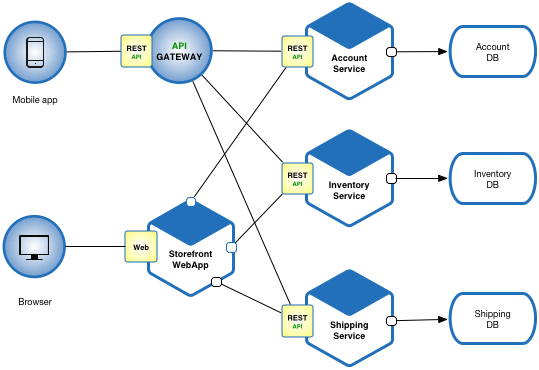
\includegraphics[width=\columnwidth]{images/Microservice_Architecture.png}
    \caption{Example of a Microservice Architecture}
\end{figure}

\subsubsection{DevOps}

The term ``DevOps'' is a mash-up between ``Development'' and ``Operations''. Two
strong and important terms in modern software engineering. The goal of DevOps is to
automate end-to-end in software development and delivery \cite{ebert:DevOps}. It enables
developers to deploy and operate their software autonomously and - in smaller teams - without
any specialized ``Ops'' department. It closes the gap between the classical
software engineers and the operations team which both had their specific tasks. DevOps
provides the means and tools to provide an agile method of software engineering with
\textit{continuous integration} and \textit{continuous deployment} \cite{huettermann:DevOps}.
